Good alignment of the SVT is critical to achieving the expected tracking performance and physics reach. 
The sensors must be aligned internally and with respect to the target and other beam line components for optimal performance. 
The alignment of the test run apparatus proceeds in several steps which must be tied together to achieve the final alignment.
These include survey measurements of various SVT assemblies, a beam line survey at JLab, and finally 
a track-based alignment. 

Optical surveys of individual modules with precision of a few microns are combined with a survey of the
overall SVT support with overall precisions of 25-100 microns to arrive at the as-built alignment.  The sag
of the long support plates and lever arms used in the test run are the dominant error in determining
relative modules positions, a defect addressed in the proposed design for the SVT.
%Mechanical surveys using touch probes was performed on the two SVT tracker planes before 
%shipping to JLab. This survey measured reference points on the base plate, C-support and on the surface of the tracker support plates. These positions where then tied to very precise optical survey of each sensor module, referencing the silicon sensor position w.r.t. to the cooling blocks. 
%An important aspect of the mechanical survey is the relatively large sag of 
%the 70~cm long support plate which is supported by the C-support hinge on one end and the 
%extension bar attached to the linear shaft at the other. The measured sag without all services 
%(cooling manifold and cables was not dressed at this point) was more than $250~\mu$m.  
%For HPS, only the first three layers are being supported from each end which will reduce this 
%sag with at least a factor of four. {\color{red} check this}. The goal of the mechanical surveys is 
%to reach a relative alignment of the 
%silicon to about $100-200~\mu$m where alignment using tracks become feasible and the 
%improvements from mechanical surveys become harder. 
After full assembly and installation of the SVT at JLab, a survey of the SVT position inside the vacuum chamber
is used to determine the location of the SVT with respect the the CEBAF beam line.

%Finally at JLab, with a fully assembled 
%tracker, an optical and touch probe survey was performed to locate 
%the SVT inside the vacuum chamber, using the measurements of the base plate, in the reference coordinate system of 
%the analyzing magnet. 

The resulting alignment is then studied using reconstructed tracks in the SVT. The main observable of the internal alignment of the silicon 
sensors is the so-called track residual. It is 
defined as the difference of the measured and predicted track 
position at that sensor. Figure~\ref{fig:res_top_nonbend} and~\ref{fig:res_top_bend} 
shows representable 3D space point track residuals, relative to track parameters determined at the target, for tracks reconstructed in the top half of the tracker.
\begin{figure*}[]
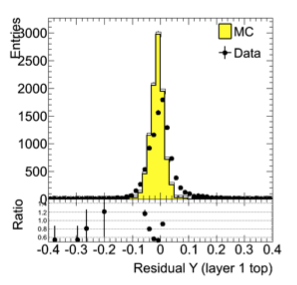
\includegraphics[ scale=1.2]{test2012/alignment/pictures/res_top/res_top-1.png}
%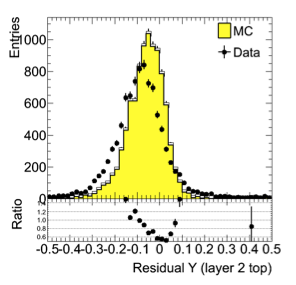
\includegraphics[ scale=0.5]{test2012/alignment/pictures/res_top/res_top-2.png}
%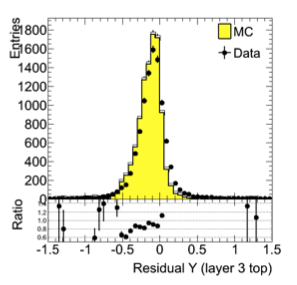
\includegraphics[ scale=0.5]{test2012/alignment/pictures/res_top/res_top-3.png}
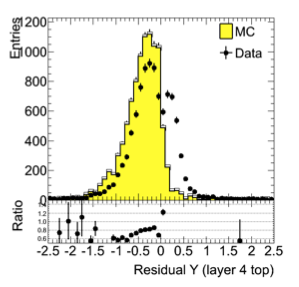
\includegraphics[ scale=1.2]{test2012/alignment/pictures/res_top/res_top-4.png}
%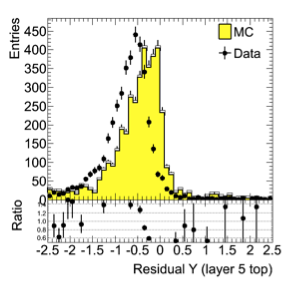
\includegraphics[ scale=0.5]{test2012/alignment/pictures/res_top/res_top-5.png}
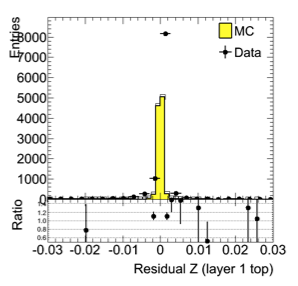
\includegraphics[ scale=1.2]{test2012/alignment/pictures/res_top/res_top-6.png}
%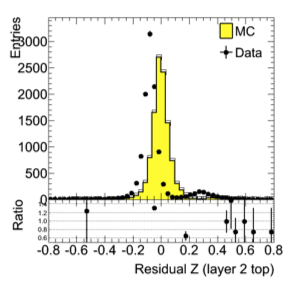
\includegraphics[ scale=0.5]{test2012/alignment/pictures/res_top/res_top-7.png}
%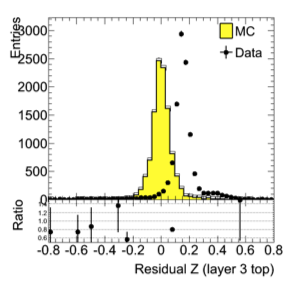
\includegraphics[ scale=0.5]{test2012/alignment/pictures/res_top/res_top-8.png}
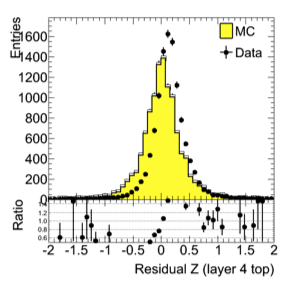
\includegraphics[ scale=1.2]{test2012/alignment/pictures/res_top/res_top-9.png}
%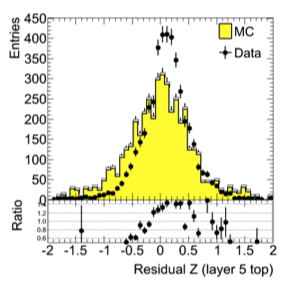
\includegraphics[ scale=0.5]{test2012/alignment/pictures/res_top/res_top-10.png}
\caption{\small{Residuals in the bend (top) and non-bend (bottom) plane 
for tracks reconstructed in the top half of the tracker after mechanical survey constants 
are applied.  }}
\label{fig:res_top_nonbend}
\end{figure*}
These are compared to the residuals from an ideally aligned tracker with residuals centered at zero.
Note the larger width for the downstream layers,highlighting the large 
multiple scattering contribution in the track reconstruction. 
%The intrinsic single hit resolution of $\approx 6~\mu$m is negligible for layers beyond the second. 
Fig.~\ref{fig:res_top_summary} shows a summary of the mean residuals for each layer of the tracker 
after the mechanical survey alignment constants have been applied.
\begin{figure*}[t]
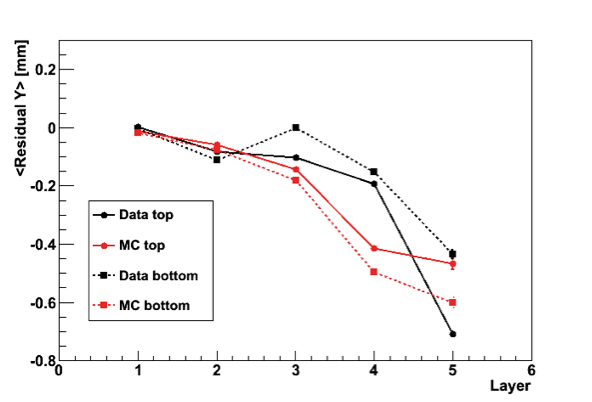
\includegraphics[ scale=0.7]{test2012/alignment/pictures/res_top/res_top_summary-1.png}
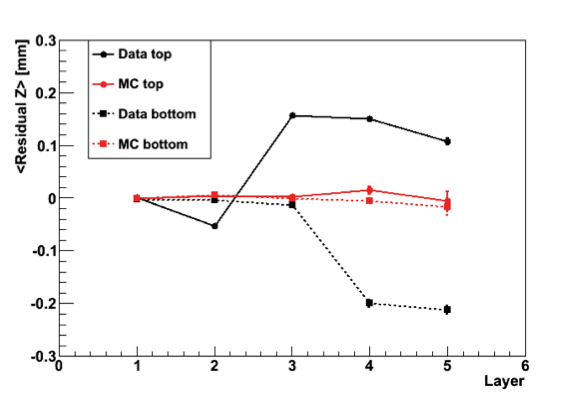
\includegraphics[ scale=0.7]{test2012/alignment/pictures/res_top/res_top_summary-2.png}\caption{\small{Mean of the track residuals for each detector layer in the top tracker half 
in the bend (left) and non-bend (right) plane after mechanical survey constants are applied.}}\label{fig:res_top_summary}
\end{figure*}
%Note that these pull distributions come from biased 
%residuals (the hit was used in the track fit) and are thus not expected to have a 
%width of one. 
%\begin{figure*}[]
%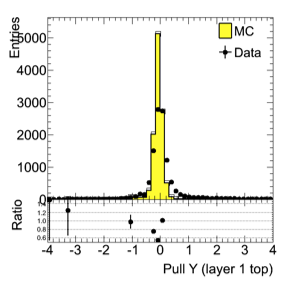
\includegraphics[ scale=1.2]{test2012/alignment/pictures/res_pull_top/res_pull_top-1.png}
%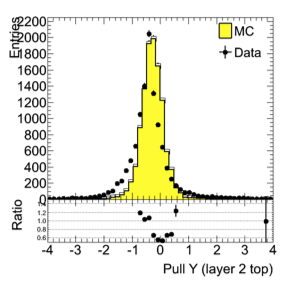
\includegraphics[ scale=0.5]{test2012/alignment/pictures/res_pull_top/res_pull_top-2.png}
%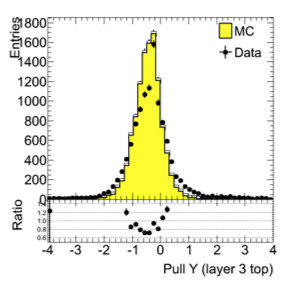
\includegraphics[ scale=0.5]{test2012/alignment/pictures/res_pull_top/res_pull_top-3.png}
%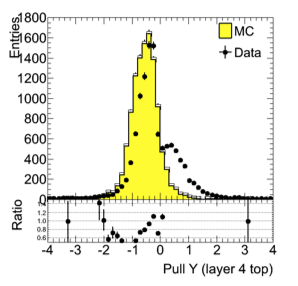
\includegraphics[ scale=1.2]{test2012/alignment/pictures/res_pull_top/res_pull_top-4.png}
%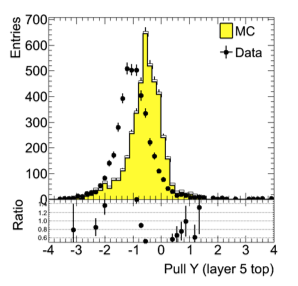
\includegraphics[ scale=0.5]{test2012/alignment/pictures/res_pull_top/res_pull_top-5.png}
%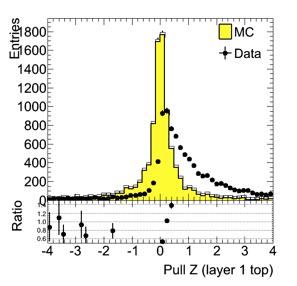
\includegraphics[ scale=1.2]{test2012/alignment/pictures/res_pull_top/res_pull_top-6.png}
%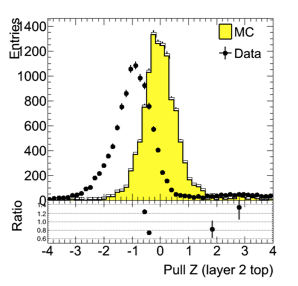
\includegraphics[ scale=0.5]{test2012/alignment/pictures/res_pull_top/res_pull_top-7.png}
%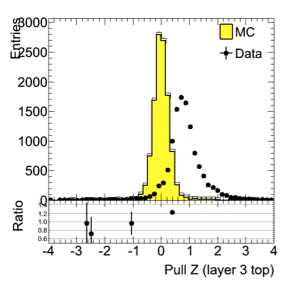
\includegraphics[ scale=0.5]{test2012/alignment/pictures/res_pull_top/res_pull_top-8.png}
%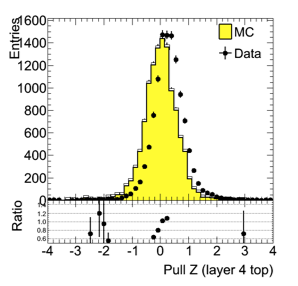
\includegraphics[ scale=1.2]{test2012/alignment/pictures/res_pull_top/res_pull_top-9.png}
%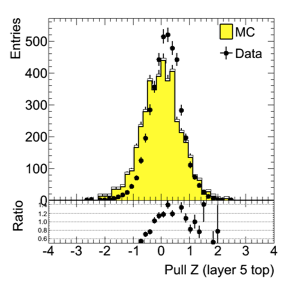
\includegraphics[ scale=0.5]{test2012/alignment/pictures/res_pull_top/res_pull_top-10.png}
%\caption{\small{Track residual pulls in the bend (top) and non-bend (bottom) plane 
%for tracks reconstructed in the 
%top half of the tracker.  }}
%\label{fig:res_pull_top_nonbend}
%\end{figure*}

To understand the tracker alignment w.r.t. to the other components on the beam line we 
use the reconstructed tracks and extrapolate them outside the tracking volume. 
Figure ~\ref{fig:extrapol_converter} shows a comparison of the track position propagated 
to the converter enabling us to get a better understanding of the tracker alignment with 
respect to the beam line. 
\begin{figure*}[t]
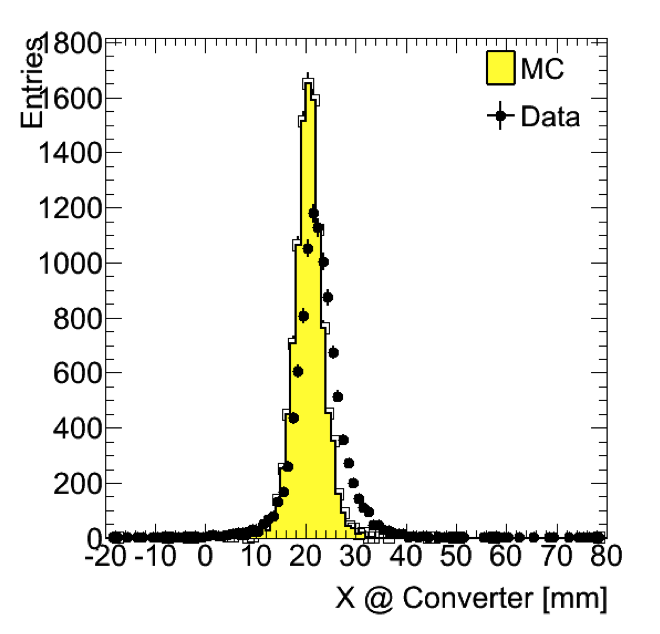
\includegraphics[ scale=0.5]{test2012/alignment/pictures/extrapolation_converter/extrapolation_X_converter_top.png}
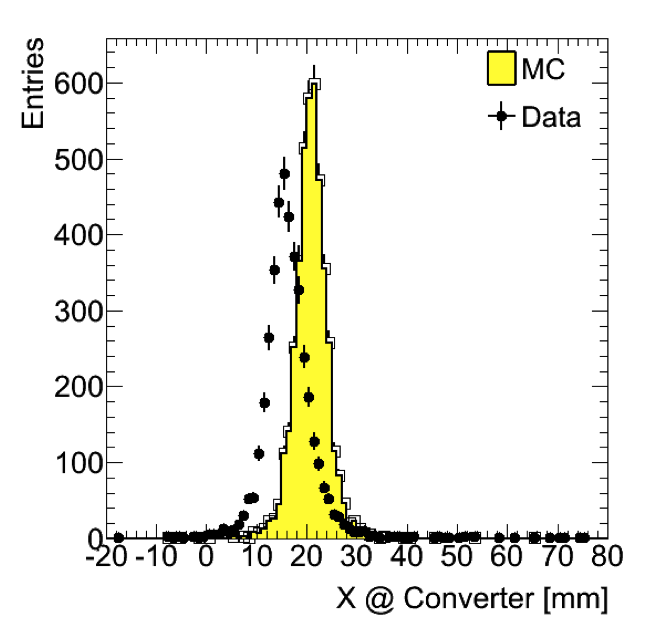
\includegraphics[ scale=0.5]{test2012/alignment/pictures/extrapolation_converter/extrapolation_X_converter_bot.png}
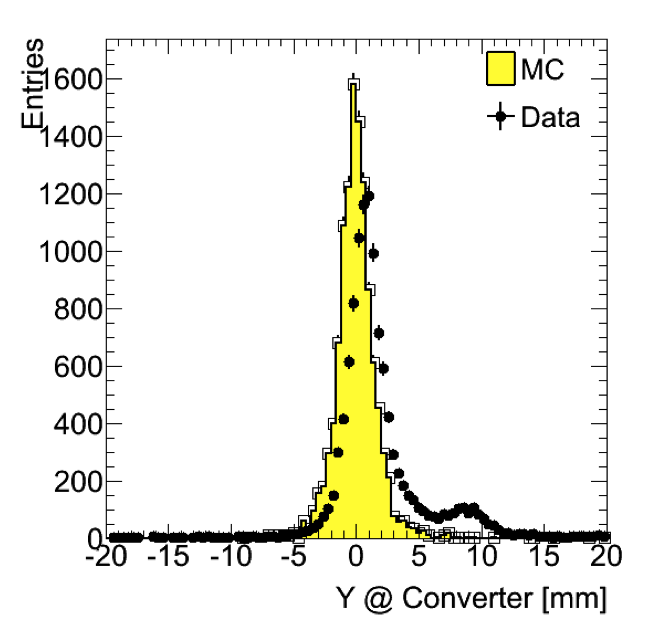
\includegraphics[ scale=0.5]{test2012/alignment/pictures/extrapolation_converter/extrapolation_Y_converter_top.png}
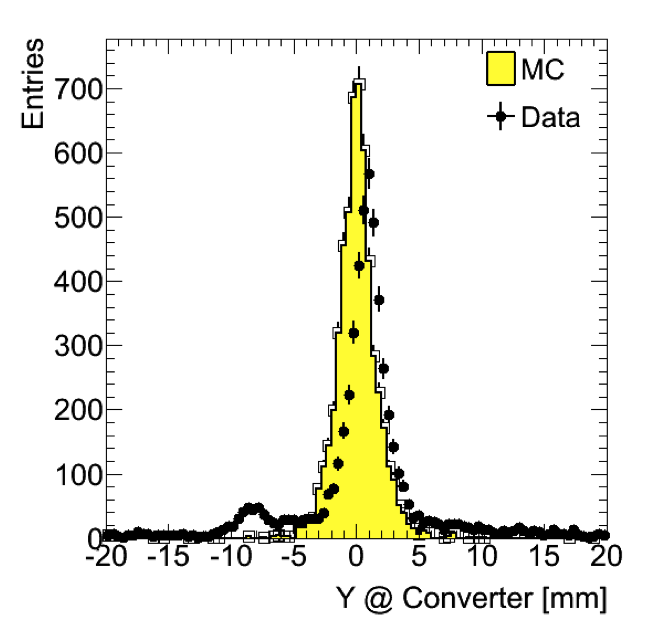
\includegraphics[ scale=0.5]{test2012/alignment/pictures/extrapolation_converter/extrapolation_Y_converter_bot.png}
\caption{\small{Extrapolated track position in the bend (top) and non-bend (bottom) 
direction for tracks reconstructed in the top (left) and bottom (right) half of the SVT. 
The extra bumps in the data at $\pm10$~mm comes from upstream backgrounds.}}
\label{fig:extrapol_converter}
\end{figure*}
The luminous region, inferred from harp scans of the photon beam profile, has a width of about 1~mm 
%(best described by a double Gaussian: $0.71e^{\frac{x}{0.366}}\times 0.29e^{\frac{x}{1.111}}$)
and a total beam envelope of around 7~mm. The small bumps in data at $\pm10$~mm 
are from particles produced upstream of the converter. The width and position of the tracks 
are roughly consistent with the expected distribution from an ideal geometry as shown by the simulated 
tracks in the same figures. The larger shift in the bend direction for bottom tracks 
is still under investigation. 

With initial residuals less than $\sim 500~\mu$m across all layers of 
the tracker and a reconstructed beam profile similar to that expected from simulation, it appears these survey techniques 
are adequate to bootstrap the SVT alignment. For HPS, we are developing 
a more sophisticated track-based alignment that delivers the best possible constants.
This framework will also enable us to explore and understand important details such as weak modes and how dedicated alignment runs 
(e.g. with magnetic field off or with different targets) may shape operational procedures during HPS running.
%Fig.~\ref{fig:test_harpscan} shows a HARP scan taken during the test run. 
%\begin{figure*}[t]
%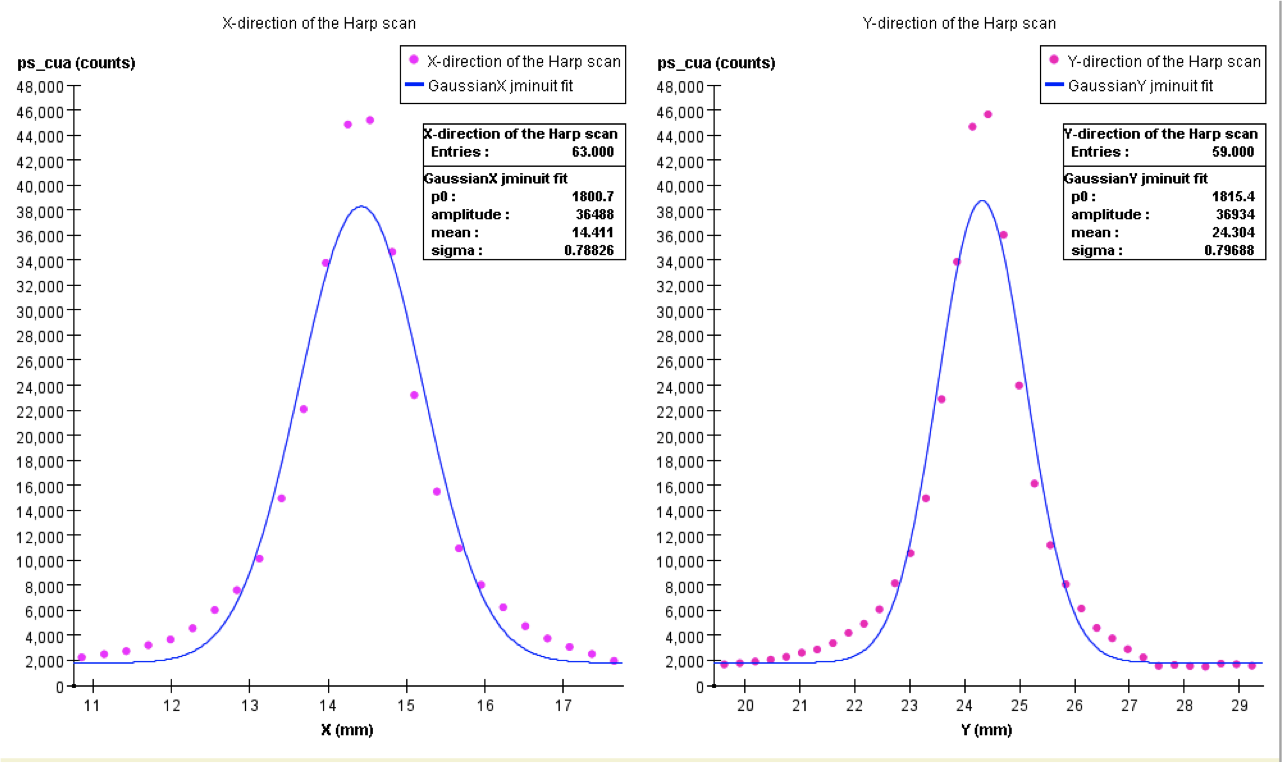
\includegraphics[ scale=0.5]{test2012/alignment/pictures/harp_scan_testrun.png}
%\caption{\small{Photon beam profile HARP scan close to the converter.}}\label{fig:testrun_harpscan}
%\end{figure*}
%The width of the beam can be described by a double Gaussian $0.71e^{\frac{x}{0.366}}\times 0.29e^{1.111}$ which is also used in the simulations. The beam envelope extends out to 
%about 7mm. 
